%%%%%%%%%%%%%%%%%%%%%%%%
%
% $Author: Deepti Hegde  $
% $Datum: 2023-06-26  $
% $Pfad: BA23-02-Sales-Predictor/report/Contents/en/Development.tex $
% $Version: 1.0 $
% $Reviewed by: Deepti, Sadegh and Raunak $
% $Review Date: 2023-07-03 $
%
%%%%%%%%%%%%%%%%%%%%%%%%


\chapter{Development}

\section{Data Selection}
The data for the forecasting the sales is downloaded from the Kaggle website. Kaggle is an online community of data scientists and machine learning practitioners. The website hosts machine learning competitions, provides datasets for research and learning purposes, and offers a platform for data science collaboration and education. It is downloaded from the link \href{https://storage.googleapis.com/kaggle-competitions-data/kaggle-v2/7391/44328/bundl}{Kaggle} using a google \ac{api}.  storage.googleapis.com is a domain used by Google Cloud Storage to store and serve user data. Google Cloud Storage is a cloud-based object storage service provided by Google, which allows users to store and access their data from anywhere on the internet.

The file is in zipped format, in which there are 7 datasets.  As you can see from the table \ref{tab:DatasetType} all datasets are in the  CSV format. CSV stands for "Comma-Separated Values." It is a file format used for storing and exchanging tabular data, such as spreadsheets or databases.

In a CSV file, each line represents a single row of data, and each column within that row is separated by a comma or other delimiter (such), such as a semicolon or a tab. The first row of a CSV file typically contains the column headers, and subsequent rows contain the data for each row.
CSV files are widely used because they are easy to create, read, and edit with a wide range of software applications, including spreadsheet programs like Microsoft Excel and Google Sheets. They are also compact, making them convenient for sharing and transferring data between different systems and platforms. 



\begin{table}[p]
	\centering
	\caption{Different types of dataset taken from Favorita stores}
	\label{tab:DatasetType}
	\begin{tabular}{|p{2cm}|p{3cm}|p{2.5cm}|p{2cm}|c|c|}
		\hline
		\textbf{Dataset} & \textbf{Description} & \textbf{Number of rows} & \textbf{Number of columns} & \textbf{Format} & \textbf{Size (KB)} \\ \hline
		train & Mainly comprises the sales figures of items based on the date, store, and product. & 125497040 & 6 & CSV & "140,000" \\ \hline
		test & Includes the identical features as the train data, except for the sales information, which we are required to forecast. & 3370464 & 5 & CSV & "126,002" \\ \hline
		stores & "Information regarding the stores, such as their type and location. & 54 & 5 & CSV & 1 \\ \hline
		items & Metadata related to the items, including their class and perishability status. & 4100 & 4 & CSV & 102 \\ \hline
		transactions & The number of sales transactions recorded in the training data & 83488 & 3 & CSV & "1,600" \\ \hline
		oil & Daily oil price & 1218 & 2 & CSV & 21 \\ \hline
		holidays\_events & Holidays in Ecuador, where some holidays are movable and can be shifted to another day (such as from the weekend to a weekday). & 350 & 6 & CSV & 22 \\ \hline
	\end{tabular}
\end{table}

The reason that the oil dataset is considered is that Ecuador's economy heavily relies on oil, making it highly susceptible to fluctuations in oil prices. All the features present in the dataset can mentioned in the table \ref{tab:DatasetFeatures} below.

\begin{table}[p]
	\centering
	\caption{Description of features in dataset}
	\label{tab:DatasetFeatures}
	\begin{tabular}{|p{2cm}|p{1.8cm}|p{3cm}|l|p{2.5cm}|}
		\hline
		\textbf{Feature} & \textbf{Datasets} & \textbf{Description} & \textbf{type} & \textbf{additional information} \\ \hline
		id & train & an identifier for the sale & int64 & ~ \\ \hline
		date & "train, transactions,  oil" & - & object & from 01.01.2017 to 15.08.2017 \\ \hline
		store nbr & "train, stores" & number of the store & int64 & 54 stores in total \\ \hline
		unit\_sales & train & "The target unit sales (e.g., 1.5 kg of cheese) - Negative values of unit\_sales represent returns of that particular item." & float64 & "range = [-15372, 89440]" \\ \hline
		onpromotion & train & tells whether that item nbr was on promotion for a specified date & bool & ~ \\ \hline
		city & stores & The city where the store is located & object & 22 cities in total \\ \hline
		state & stores & The state where the store is located & object & 16 states in total \\ \hline
		type & stores & the type of store & object & ~ \\ \hline
		cluster & stores & a grouping of similar stores & int64 & 17 different clusters \\ \hline
		family & items & the family which an item belongs to & holidays\_events & "takes values such as: 'BREAD/BAKERY', 'EGGS', 'MEATS'" \\ \hline
		class & items & the class which an item belongs to & int64 & 337 classes in total \\ \hline
	\end{tabular}
\end{table}

\begin{table}[p]
	\centering
	\begin{tabular}{|p{2cm}|p{1.9cm}|p{3cm}|p{3cm}|p{2.5cm}|}
		\hline
		\textbf{Feature} & \textbf{Datasets} & \textbf{Description} & \textbf{type} & \textbf{additional information} \\ \hline
		persihable & items & shows if an item is persihable or not & int64 & 0 for nonperishable and 1 for perishable (could be read as bool) \\ \hline
		transaction & transactions & The count of transactions & int64 & "range = [5, 8359]" \\ \hline
		dcoilwtico & oil & Crude oil prices & float64 & "range = [26.19, 110.62], standard deviation = 25.63" \\ \hline
		type & holiday\_events & type of the holiday & object & 6 types in total \\ \hline
		locale & holiday\_events & "Shows if the holiday is local, regional, or national" & object & ~ \\ \hline
		locale\_name & holiday\_events & Shows the name of the location where the holiday is celebrated & object & ~ \\ \hline
		description & holiday\_events & description of the holiday & object & ~ \\ \hline
		transferred & holiday\_events & shows if a holiday is transferred or not & bool & ~ \\ \hline
	\end{tabular}
\end{table}

\section{Data Preparation}

	The goal of data preparation step is to improve the quality of the selected data. 
	
	Previously, the dataset contained a substantial amount of data, resulting in a large file size of 5GB. To address this, a filtering process was implemented to extract the data specifically for the year 2017. Our code utilized a date mask to select data falling within the range of '2017-01-1' to '2017-08-15'. It then assigned the filtered data to a dataframe named salesdf and exported it to a CSV file named 'salesdf\_masked.csv'.
	
	After the initial data reduction process, the resulting dataset now only contains the data for the year 2017. As a result, the dataset's size has significantly decreased from 5GB to a mere 140MB, representing an impressive reduction in file size.
	
	This achievement brings several advantages, including improved storage efficiency and enhanced data processing speed, allowing for more effective utilization of the dataset in subsequent analyses or operations.
	
	\textbf{Data Quality}
	Data quality refers to the accuracy, completeness, and consistency of data. In other words, it is the degree to which data is fit for its intended purpose in operations, decision-making, and planning.
	
	\textbf{Anomalies}
	Data anomalies are any unexpected or inconsistent observations or patterns in a dataset that deviate from the norm or expected behavior. Data anomalies can take many forms, including outliers, missing values, and duplicate records. Anomalies can also be caused by changes in the underlying data-generating process or by unusual patterns or trends in the data that are not readily explained by known factors.
	
	\textbf{Data Completeness}
	There is a description of the number of missing values in the data sets can be seen in the table \ref{tab:DatasetMissing}:
	
	\begin{table}[h!]
		\centering
		\caption{Description of missing values in the dataset}
		\label{tab:DatasetMissing}
		\begin{tabular}{|l|l|p{3cm}|p{3cm}|}
			\hline
			\textbf{Dataset} & \textbf{Feature} & \textbf{Number of missing values} & \textbf{Measure of completeness (\%)} \\ \hline
			train & onpromotion & 21657651 & 86.7 \\ \hline
			oil & dcoilwtico & 43 & 96.5 \\ \hline
		\end{tabular}
	\end{table}
	
	There are no missing values in other datasets. Completeness is measured by dividing the number of NA values and dividing by the number of complete values in the same column. NA values, or "missing values," are data points that are not available or are unknown. In other words, they are values that are not present in a data. NA stands for “Not Available”.
	
	\textbf{Outliers}
	Outliers in data refer to data points that are significantly different from other data points in the same dataset. They can be defined as observations that fall outside the typical range of values for a given variable.
	
	\textbf{Interquartile range method}
	The range of the middle 50\% of a dataset can be determined using the interquartile range (IQR). By setting up "fences" based on the IQR, data points outside of these boundaries can be classified as outliers.
	To identify outliers in a dataset using the interquartile range (IQR) method, you can follow these steps:
	\begin{align*}
		\text{Q1} &= \text{25th percentile} \\
		\text{Q3} &= \text{75th percentile} \\
		\text{IQR} &= \text{Q3} - \text{Q1} \\
		\text{Upper fence} &= \text{Q3} + (1.5 \times \text{IQR}) \\
		\text{Lower fence} &= \text{Q1} - (1.5 \times \text{IQR})
	\end{align*}
	
	Use your fences to highlight any outliers, all values that fall outside your fences. 
	
	Outliers are any values greater than your upper fence or less than your lower fence.
	
	The overview of outliers in our dataset can be seen in the table \ref{tab:DatasetOutliers}
	\begin{table}[h!]
		\centering
		\caption{Overview of outliers in the dataset}
		\label{tab:DatasetOutliers}
		\begin{tabular}{|l|l|l|p{3cm}|}
			\hline
			\textbf{Dataset} & \textbf{Feature} & \textbf{Number of Outliers} & \textbf{Measure of completeness (\%)} \\ \hline
			train & Unit\_sales & 11497596 & 86.7 \\ \hline
			transactions & transactions & 4583 & 96.5 \\ \hline
		\end{tabular}
	\end{table}
	
	In our cases, outliers are legitimate data points that are indicative of rare events or extreme values in the data. It may be appropriate to keep the outliers in the dataset.
	
	\textbf{Data Uniqueness}
	To measure uniqueness of the datasets, number of duplicate values are calculated. Duplicate values in data refer to observations or rows in a dataset that have identical values across all variables or columns. There are no duplicate values in any of the datasets presented, so uniqueness measure for all the datasets is 100\%.
	
	\textbf{Fairness and Bias}
	Bias can occur in many ways, such as through sampling bias, selection bias, or measurement bias. It's essential to identify potential sources of bias and assess their impact on the data. Once the potential sources of bias are identified, it's important to evaluate their impact on the data. 
	One way to identify fairness/bias is to check if the missing values in the data have a pattern to them or  are missing at random. The missing values in the "train" dataset in the "onpromotion" feature do not exist at random, as they are all in the first rows of the data. So it could be mentioned that there is some bias in this dataset. In contrast, the missing values in the oil dataset in the "dcoilwtico" feature seem to be happening at random. Although, it is not clear whether it was done deliberately or not, which is beyond this study.
	Outliers can also have a significant impact on the analysis and be a source of bias in the data. They may need to be handled appropriately. But as mentioned before, outliers are legitimate data points in our case and we do not consider the as a source of bias. 


\section{Data Transformation}

\subsection{One Hot Encoding}

One Hot Encoding is a data transformation technique used in machine learning and data analysis to represent categorical variables as binary vectors \cite{Harris:2015}. It is often employed when working with categorical data that cannot be directly used in mathematical models or algorithms.

In One Hot Encoding, each category is transformed into a binary vector where all elements are zero except for the index that represents the corresponding category, which is set to one. This conversion allows the categorical data to be interpreted and used in numerical computations.

Here's an example to illustrate how One Hot Encoding works:

Suppose we have a dataset with a categorical feature called "Color" that can take three values: "Red," "Green," and "Blue." To apply One Hot Encoding, we create three binary columns, one for each unique category. The columns are then populated as follows:

\begin{center}
	\begin{tabular}{|c|c|c|c|}
		\hline
		Color & Color\_Red & Color\_Green & Color\_Blue \\
		\hline
		Red   & 1         & 0            & 0           \\
		Green & 0         & 1            & 0           \\
		Blue  & 0         & 0            & 1           \\
		\hline
	\end{tabular}
\end{center}

In this example, the original "Color" column is replaced by three new columns, "Color\_Red," "Color\_Green," and "Color\_Blue." Each column represents one category, and the value in each column indicates whether the corresponding category is present or not.

One Hot Encoding allows categorical variables to be used in machine learning models that require numerical input, such as regression or neural networks [\cite{Jie:2019}]. It avoids introducing an arbitrary order or numerical relationship between the categories, which could mislead the model.

\subsection{Why Use a One Hot Encoding?}

One Hot Encoding is used for several reasons in machine learning and data analysis:

\begin{enumerate}
	\item Handling Categorical Variables: Many machine learning algorithms and models are designed to work with numerical data. However, real-world datasets often contain categorical variables, such as gender, color, or product categories. One Hot Encoding allows us to represent categorical variables as numerical features that can be effectively used by these models.
	
	\item Preserving Categorical Information: One Hot Encoding preserves the categorical information without introducing any ordinal relationship or numerical assumptions between the categories. By using binary vectors, each category is represented as a distinct feature, and the absence or presence of a category is explicitly indicated by the corresponding binary values.
	
	\item Avoiding Misinterpretation: If categorical variables were simply encoded with arbitrary numerical values (e.g., assigning integers to categories), it could mislead the model into assuming an inherent order or magnitude among the categories. One Hot Encoding eliminates this potential misinterpretation by representing each category as an independent binary feature.
	
	\item Enhancing Model Performance: One Hot Encoding can improve the performance of machine learning models by providing them with more relevant and precise information about the categorical variables. Models can learn and capture the relationships and patterns associated with each category separately, leading to better predictive accuracy.
	
	\item Compatibility with Algorithms: Many machine learning algorithms, such as linear regression, logistic regression, support vector machines, and neural networks, require numerical input features. One Hot Encoding enables categorical variables to be used seamlessly with these algorithms, enabling the utilization of the full dataset in the learning process.
	
	\item Handling High Cardinality: One Hot Encoding is particularly useful when dealing with categorical variables that have high cardinality, meaning they have a large number of unique categories. Instead of creating a single column with multiple distinct values, One Hot Encoding breaks down the variable into multiple binary features, making it more manageable for the model to process.
	
\end{enumerate}

One Hot Encoding is utilized to transform categorical variables into numerical representations that can be effectively utilized by machine learning models. It ensures the preservation of categorical information, avoids misinterpretation, enhances model performance, ensures compatibility with algorithms, and handles high cardinality variables.

\subsection{One Hot Encoding Deployment}

As can be seen in the Listing \ref{one-hot-encoding} below, one hot encoding is done using the \lstinline{get_dummies} function in the \lstinline{pandas} library. This is  done on the specified variables in the \lstinline{Salesdf_filtered} DataFrame and adds the resulting dummy variables as new columns. It then removes the original variables and the \lstinline{year} column from the DataFrame.


\begin{lstlisting}[label=one-hot-encoding, caption=One hot encoding using get\_dummies on pandas dataframe]
	## One hot encoding using get_dummies on pandas dataframe.
	dummy_variables = ['onpromotion','city','type_x','cluster','store_nbr','item_nbr',
	'family','perishable','type_y', 'locale', 'transferred', 'month', 'day']
	
	for var in dummy_variables:
	dummy = pd.get_dummies(Salesdf\_filtered[var], prefix = var, drop\_first = False)
	Salesdf\_filtered = pd.concat([Salesdf\_filtered, dummy], axis = 1)
	
	Salesdf\_filtered = Salesdf\_filtered.drop(dummy\_variables, axis = 1)
	Salesdf\_filtered = Salesdf\_filtered.drop(['year'], axis = 1)
\end{lstlisting}

in the Figure \ref{Fig:Transformation} you cans see the first 5 rows of the \lstinline{Salesdf_filtered}:

\begin{center}
	\begin{figure}[h!]
		\begin{center}
			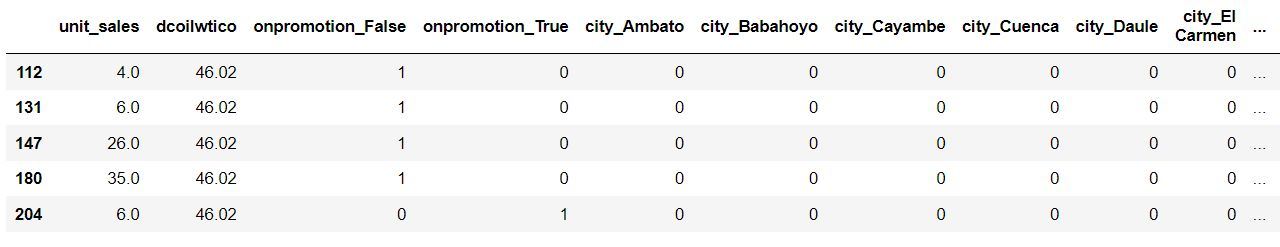
\includegraphics[height=30mm, width=130mm]{Images/Transformation}
		\end{center}
		\caption{The above dataframe contains data after the one hot encoding technique is applied to the data.} 
		\label{Fig:Transformation}
	\end{figure}
\end{center}

Caption: The above dataframe contains data after the one hot encoding technique is applied to the data.

Rescaling of the \lstinline{'unit_sales'} and \lstinline{'dcoilwtico'} variables in the \lstinline{Salesdf_filtered} DataFrame is done as shown in the Listing \ref{lst:rescaling}. It calculates the minimum and maximum values of the \lstinline{'unit_sales'} column and assigns them to \lstinline{min_train} and \lstinline{max_train}, respectively. Then, for each variable in the \lstinline{scalable_variables} list, it calculates the minimum and maximum values of that variable in the DataFrame. It rescales each variable by subtracting the minimum value and dividing by the range (\lstinline{max - min}). The rescaled values are then updated in the DataFrame. This rescaling process ensures that the variables are normalized within a certain range, which can be useful for further analysis or modeling.


\begin{lstlisting}[language=Python, caption={Re-scaling of variables}, label={lst:rescaling}]
	# Re-scale
	# We keep this value to re-scale the predicted unit_sales values in the following lines of code.
	min_train, max_train = Salesdf_filtered['unit_sales'].min(), Salesdf_filtered['unit_sales'].max()
	
	scalable_variables = ['unit_sales','dcoilwtico']
	
	for var in scalable_variables:
	mini, maxi = Salesdf_filtered[var].min(), Salesdf_filtered[var].max()
	Salesdf_filtered.loc[:,var] = (Salesdf_filtered[var] - mini) / (maxi - mini)
\end{lstlisting}

The code in Listing \ref{lst:train-database} prepares the training database by removing the \lstinline{'unit_sales'} column from the \lstinline{Salesdf_filtered} DataFrame. First, it resets the index of the DataFrame to ensure a consecutive sequence starting from 0 using \lstinline{reset_index(drop=True)}. Then, it assigns the values of the \lstinline{'unit_sales'} column to the variable \lstinline{y}, representing the target variable that we want to predict. Finally, it creates the feature variable dataset \lstinline{X} by dropping the \lstinline{'unit_sales'} column from the DataFrame using \lstinline{drop(['unit_sales'], axis=1)}. This code separates the target variable from the feature variables, allowing us to use \lstinline{X} as the input data and \lstinline{y} as the corresponding target values for training machine learning models to predict \lstinline{unit_sales} based on the remaining features.



\begin{lstlisting}[language=Python, caption={Preparing the training database}, label={lst:train-database}]
	# train database without unit_sales
	Salesdf_filtered = Salesdf_filtered.reset_index(drop=True)  # we reset the index
	y = Salesdf_filtered['unit_sales']
	X = Salesdf_filtered.drop(['unit_sales'], axis=1)
\end{lstlisting}



The code in Listing \ref{lst:train-test-split} performs a train-test split on the dataset for machine learning purposes. The variable \lstinline{num_test} is set to 0.20, indicating that 20\% of the data will be allocated for testing. The \lstinline{train_test_split} function is then used to split the feature variables \lstinline{X} and the target variable \lstinline{y} into \lstinline{X_train} (training set for features), \lstinline{X_test} (testing set for features), \lstinline{y_train} (training set for target variable), and \lstinline{y_test} (testing set for target variable). The \lstinline{test_size} parameter is set to \lstinline{num_test} to specify the proportion of the data allocated for testing, and the \lstinline{random_state} parameter is set to 15 for reproducibility of the split. 

\begin{lstlisting}[language=Python, caption={Train-test split of the dataset}, label={lst:train-test-split}]
	num_test = 0.20
	X_train, X_test, y_train, y_test = train_test_split(X, y, test_size=num_test, random_state=15)
\end{lstlisting}

the train and test set sizes are given in the Table \ref{tab:data-split}. As can be seen from this table, it is confirmed that 20\% of the rows are allocated to the test sets. 


\begin{table}[!h]
	\centering
	\caption{Train and Test Set Sizes}
	\label{tab:data-split}
	\begin{tabular}{|l|p{3cm}|p{3cm}|}
		\hline
		\textbf{Dataset} & \textbf{Number of Samples (Rows)} & \textbf{Number of Features (Columns)} \\
		\hline
		X\_train & 27365 & 147 \\
		y\_train & 27365 & - \\
		X\_test & 6842 & 147 \\
		y\_test & 6842 & - \\
		\hline
	\end{tabular}
\end{table}


\bigskip







	


\section{Data Mining}
Data Mining: is a step in the KDD process consisting of applying computational techniques that, under acceptable computational efficiency limitations, produce a particular enumeration of patterns (or models) over the data. It is concerned with the algorithmic means by which patterns are extracted and enumerated from data.

Typical methods of data mining are:

\begin{itemize}
	\item \textbf{Cluster Analysis:} Grouping of objects based on similarities
	\item \textbf{Classification}: Elements are assigned to existing classes
	\item \textbf{Association Analysis}: Identification of correlations and dependencies in data
	\item \textbf{Regression Analysis}: Identification of relationships between variables
	\item \textbf{Outlier Detection}: Identification of unusual data sets
	\item \textbf{Correlation Analysis}: Examines the relationship between two variables
	\item \textbf{Summary}: Transformation of the data set into a more compact description without significant 		loss of information.
\end{itemize}


We have choosen regression analysis for our model because practice shows that the use of regression approaches can often give us better results compared to time series methods. One of the main assumptions of regression methods is that the patterns in the past data will be repeated in future \cite{Pavlyshenko:2019}.



\section{Model}
We have identified seven models i.e. Linear regression, Decision Tree regression, Extra Tree regresision, Random Forest Regression, Gradient Boosting Regression, XG Boost, and \ac{LGBM} for regression analysis.

\begin{enumerate}
	
	\item \textbf{Creating a Neural Network:}
	Multi-layer Perceptron (MLP) is a supervised learning algorithm that learns a function by training on a dataset, where is the number of dimensions for input and is the number of dimensions for output. The advantages of Multi-layer Perceptron are:
		\begin{itemize}
			\item Capability to learn non-linear models.
	
			\item Capability to learn models in real-time (on-line learning) using partial\_fit.
			
			 \begin{lstlisting}[language=Python]
				# Convert data as np.array
				features = np.array(X_train)
				#targets = np.array(y_train.reshape(y_train.shape[0],1))
				targets = np.array(y_train.values.reshape(y_train.shape[0],1))
				features_validation= np.array(X_test)
				#targets_validation = np.array(y_test.reshape(y_test.shape[0],1))
				targets_validation = np.array(y_test.values.reshape(y_test.shape[0],1))
				
				print(features[:10])
				print(targets[:10])
			\end{lstlisting}
			
		\end{itemize}
	
		\item \textbf{Splitting the dataset into Training and Validation:}
		
		The dataset split for training is 80\% and that for validation is 20\%
		
		 \begin{lstlisting}[language=Python]
			# Split the data into training and validation sets
			features_train, features_validation, targets_train, targets_validation = train_test_split(
			features, targets, test_size=0.2, random_state=42)
			
			# Defining the model
			model = Sequential()
			model.add(Dense(64, input_dim=features.shape[1], activation='relu'))
			model.add(Dense(32, activation='relu'))
			model.add(Dense(1, activation='linear'))
			model.compile(loss='mean_squared_error', optimizer='adam', metrics=['mean_squared_error'])
			
			# Training the model
			epochs_tot = 1000
			epochs_step = 250
			epochs_ratio = int(epochs_tot / epochs_step)
			hist = np.array([])
			
			for i in range(epochs_ratio):
			history = model.fit(features_train, targets_train, epochs=epochs_step, batch_size=100, verbose=0)
			
			# Evaluate the model on the training and validation sets
			print("Step: ", i * epochs_step, "/", epochs_tot)
			train_mse = model.evaluate(features_train, targets_train, verbose=0)[1]
			print("Training MSE:", train_mse)
			val_mse = model.evaluate(features_validation, targets_validation, verbose=0)[1]
			print("Validation MSE:", val_mse, "\n")
			
			# Append the MSE values to the history array
			hist = np.concatenate((hist, np.array(history.history['mean_squared_error'])), axis=0)
		\end{lstlisting}
	
	
	\item \textbf{Linear Regression:}
	 Linear Regression is a linear approach for modelling the relationship between a scalar dependent variable y and one or more explanatory variables (or independent variables) denoted X. The case of one explanatory variable is called simple linear regression. For more than one explanatory variable, the process is called multiple linear regression.
	 
	 Linear regression models are often fitted using the least squares approach, but they may also be fitted in other ways, such as by minimizing the "lack of fit" in some other norm (as with least absolute deviations regression), or by minimizing a penalized version of the least squares cost function as in ridge regression (L2-norm penalty) and lasso (L1-norm penalty).
	 
	 \begin{lstlisting}[language=Python]
	 	# Fit the linear model
	 	model = linear_model.LinearRegression()
	 	results = model.fit(X_train, y_train)
	 	print(results)
	 \end{lstlisting}
 
 	\item \textbf{Decision Tree Regression:}
 	A decision tree is a decision support tool that uses a tree-like graph or model of decisions and their possible consequences, including chance event outcomes, resource costs, and utility. It is one way to display an algorithm that only contains conditional control statements. For Decision Tree Regression, the R2 score is 0.34 and MSE score is 0.0006.
 	
 	 \item \textbf{Extra Trees Regression:}
 	Extra-trees differ from classic decision trees in the way they are built. When looking for the best split to separate the samples of a node into two groups, random splits are drawn for each of the max\_features randomly selected features and the best split among those is chosen. For Extra Trees Regression, the R2 score is 0.756 and MSE score is 0.00023.
 	
 	 \item \textbf{Random Forest Regression:}
 	Random forests or random decision forests are an ensemble learning method for classification, regression and other tasks, that operate by constructing a multitude of decision trees at training time and outputting the class that is the mode of the classes (classification) or mean prediction (regression) of the individual trees.Random decision forests correct for decision trees' habit of overfitting to their training set. For Random Forrest Regression, the R2 score is 0.839 and MSE score is 0.00015.
 	
 	 \item \textbf{Gradient Boosting Regression:}
 	The idea of boosting came out of the idea of whether a weak learner can be modified to become better. A weak hypothesis or weak learner is defined as one whose performance is at least slightly better than random chance. Hypothesis boosting was the idea of filtering observations, leaving those observations that the weak learner can handle and focusing on developing new weak learns to handle the remaining difficult observations. For Gradient Boosting Regression, the R2 score is 0.839 and MSE score is 0.00015.
 	
 	\item \textbf{XG Boost:}
 	XGBoost (eXtreme Gradient Boosting) is a direct application of Gradient Boosting for decision trees. Main advantages are as follows:
 		\begin{itemize}
 			\item Easy to use
 			\item Computational efficiency
 			\item Model Accuracy
 			\item Feasibility, easy to tune parameters and modify objectives.
 		
 		\end{itemize}
 	
 	For XG Boost, the R2 score is 0.858 and MSE score is 0.00013.
 	
 		\item \textbf{LGBM:}
			Light GBM is a fast, distributed, high-performance gradient boosting framework based on decision tree algorithm, used for ranking, classification and many other machine learning tasks. Since it is based on decision tree algorithms, it splits the tree leaf wise with the best fit whereas other boosting algorithms split the tree depth wise or level wise rather than leaf-wise. So when growing on the same leaf in Light GBM, the leaf-wise algorithm can reduce more loss than the level-wise algorithm and hence results in much better accuracy which can rarely be achieved by any of the existing boosting algorithms. For LGBM, the R2 score is 0.819 and MSE score is 0.00021.

\end{enumerate}


\section{Evaluation}

\textbf{Performance Analysis of Prediction}
The performance evaluation of any regression algorithm involves providing the test data to the training model. This process assesses how well the model has learned the underlying patterns in the dataset and its ability to predict values for new data. The performance of a regression model can be measured using either the Mean Square Error (MSE) or the R2 error. \cite{krishna:2018}
The MSE is calculated using the following formula:

\[MSE = \frac{1}{n}\sum_{i=1}^{n}(y_i - \hat{y}_i)^2\]

Where \(y_i\) represents the predicted value and \(\hat{y}_i\) represents the corresponding value from the dataset.

The R2 error is calculated using the following formula:

\[R^2 = 1 - \frac{SS_{res}}{SS_{tot}}\]

Where \(SS_{res}\), known as the residual sum of squares, is calculated as:

\[SS_{res} = \sum_{i=1}^{n}(y_i - \hat{y}_i)^2\]

And \(SS_{tot}\), referred to as the total sum of squares, is calculated as:

\[SS_{tot} = \sum_{i=1}^{n}(\hat{y}_i - \bar{y})^2\]

Here, \(\bar{y}\) represents the mean of the observed data, which is computed as:

\[\bar{y} = \frac{1}{n}\sum_{i=1}^{n}y_i\]

Table \ref{tab:model-performance} provides a comparison of different regression models based on their performance metrics: R2 $(R^2)$ Score and MSE Score.

The R2 Score represents the coefficient of determination, indicating the proportion of the variance in the dependent variable that can be explained by the independent variables. Higher values of R2 Score indicate a better fit of the model to the data.

The MSE Score, or Mean Squared Error, measures the average squared difference between the predicted and actual values. Lower MSE Scores indicate better model performance with smaller prediction errors.


\begin{table}[h]
	\caption{Regression Model Performance}
	\label{tab:model-performance}
	\centering
	\begin{tabular}{|l|c|c|}
		\hline
		\textbf{Model} & \textbf{R2 Score} & \textbf{MSE Score} \\
		\hline
		Linear Regression & 0.366 & NaN \\
		Decision Tree Regression & 0.342 & 0.00061 \\
		Extra Tree Regression & 0.756 & 0.00023 \\
		Random Forest Regression & 0.839 & 0.00015 \\
		Gradient Boosting Regression & 0.839 & 0.00015 \\
		XG Boost & 0.858 & 0.00013 \\
		LGBM & 0.819 & 0.00021 \\
		\hline
	\end{tabular}
\end{table}

The XG Boost model emerged as the top performer among the regression models, boasting the highest R2 Score and the lowest MSE Score. This indicates that XG Boost provides the best overall fit to the data and generates highly accurate predictions. Its superior performance suggests that it captures a larger portion of the underlying patterns and relationships within the dataset, making it a reliable choice for regression tasks.

The Random Forest Regression and Gradient Boosting Regression models also demonstrated strong performance, with both achieving impressive R2 Scores and low MSE Scores. These models showcased their ability to effectively capture and utilize the complex interactions among the predictors to make accurate predictions.



